\documentclass[6pt]{scrartcl}
\usepackage[landscape,margin=20pt]{geometry}

\usepackage{amsmath}
\usepackage{amssymb}
\usepackage{multicol}
\usepackage{graphicx}
\usepackage{setspace}
\usepackage[compact]{titlesec}

\usepackage{hyperref}
\hypersetup{
    colorlinks,%
    citecolor=black,%
    filecolor=black,%
    linkcolor=black,%
    urlcolor=black
}

\graphicspath{{img/}}


%Commands to format and shorten
\setlength{\columnseprule}{0.1pt}
\setlength{\parindent}{0cm}
\setlength{\parskip}{0em plus 0.2em minus 0.2em}%plus 0.1ex minus 0.2ex}

\pagestyle{empty} 



\begin{document}
\begin{multicols}{4}
\section{Introduction}
\subsection{Protocol performances}
$G$: Total load, $S$ arrival rate of new packets. 
\subsubsection{Pure ALOHA} If you have data to send, send the data. If the message collides with another transmission, try resending later. On collision, sender waits random time before trying again.
$P(k \text{ transm. in } 2X\text s) = \frac{(2G)^k}{k!} e^{-2G}$\\
$S = G \cdot P(0) = Ge^{-2G}$


\subsubsection{Slotted ALOHA} 
%C'est pas slotted alpha ça? 
Probability of $k$ packets generated during a slot:
$P(k) = \frac{G^ke^{-G}}{k!}$
Throughput:
$P(1) = Ge^{-G}$

\subsubsection{CSMA}
Goal: reduce the wastage of bandwidth due to packet collisions.
Principle: sensing the channel before transmitting (never transmit when the channel is busy).
\paragraph{Non-persistent} If channel is busy, directly run back off algorithm.
\paragraph{p-persistent} If it is busy, they persist with sensing until the channel becomes idle. If it is idle:\\
- With probability $p$, the station transmits its packet\\
- With probability $1-p$, the station waits for a random time and senses again

\paragraph{Performance of Unslotted nonpersistent CSMA}:
For $a=t_\textrm{prop}/X$, the normalized one-way propagation delay.
$S = \frac{G^{-aG}}{G(1+2a)+e^{-aG}}$

\paragraph{Performance of Slotted nonpersistent CSMA}:
$S = \frac{aG^{-aG}}{1-e^{-aG} + a}$

\includegraphics[height=\columnwidth, angle=270]{comparatif}

\subsection{Exercises}
Capacity of a link vs Transmission capacity (=total capacity of all the links). Wire : $C_t=\min \{C_1, C_2\}$ Wireless : $d/C_t = d/C_1+d/C_2 \leftrightarrow C_t = (c_1 c_2/c_1+c_2)$\\
ALOHA : Aloha channel with infinite number of users gives 94\% of idle slots. $P(0) = \mathrm{e}^{-G}=0.94 \rightarrow G=0.062$ \\ $S=P(1)=G\mathrm{e}^{-G}\approx 5.8\%$ \\ $G<G_{peak} = 1$ : channel underloaded. \\ Ration of busy slots occupied by collisions : $\frac{1-P(0)-P(1)}{1-P(0)}=3.3\%$

\section{WLAN Engineering aspects}
\includegraphics[width=\columnwidth]{frequencies}
Frequency(f) and wave length($\lambda$), $c=3 \times 10^8 m/s$  : $\lambda = c/f$
\subsection{802.11}
\textbf{Physical layer} : DSSS or FHSS,
\textbf{MAC Layer} : best effort asynchronous data service, DCF CSMA/CA (mandatory), DCF with RTS/CTS or PCF (optional)
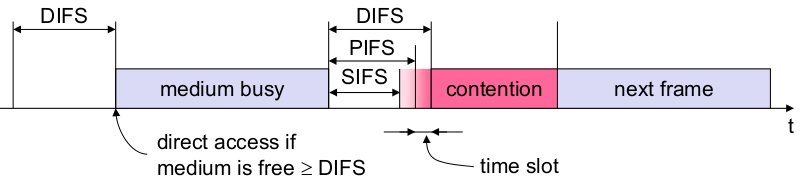
\includegraphics[width=\columnwidth]{B1}
CSMA/CA Unicast : \\
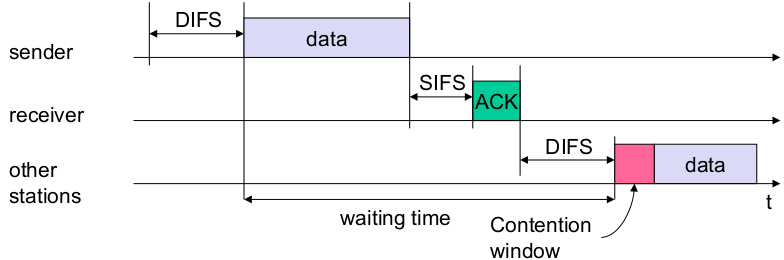
\includegraphics[width=\columnwidth]{B12}
DCF with RTS/CTS (with fragmentation) : \\
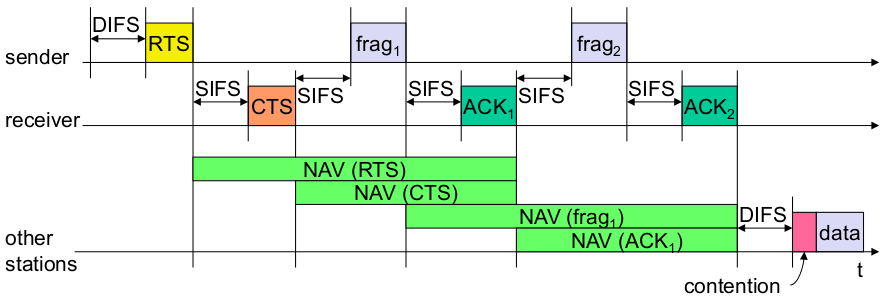
\includegraphics[width=\columnwidth]{B14}
MAC address format : \\
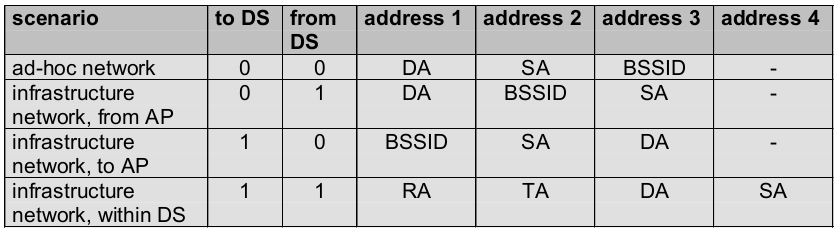
\includegraphics[width=\columnwidth]{B15}
\subsection{Exercises}
Wireless LAN use polling between M workstations and a central access point. Channel at 25Mbps. Stations 100 m away from AP, polling messages 64 bytes long. Packet length : 1250 bytes. No more packet indicated with 64-byte message. Maximum arrival rate $\lambda_{max} = \rho_{max} * Br/P_{length}$ $\rho_{max}=\frac{Effective time}{Whole time}=\frac{M*N*T_{packet}}{M*(NT_{packet}+T_{poll}+T_{end}+2t_{prop})}$ $t_{prop}=d/c$ $T_{packet}=\frac{1250*8}{25*10^6}$\\
One station A sends a frame to another station B in a different BSS in
an IEEE 802.11 infrastructure network with DCF access method without RTS/CTS.
\\
A $\rightarrow$ AP1 \\
\begin{tabular}{|c|c|c|c|c|c|c|}
  \hline
  To & From & Type & Dur & A1 & A2 & A3 \\
  \hline
  1 & 0 & Data & $T_{d}+SIFS+T_{A}$ & BSS1 & A & B \\
  \hline
\end{tabular}\\
AP1 $\rightarrow$ A\\
\begin{tabular}{|c|c|c|c|c|}
  \hline
  To DS & From DS & Type & Duration & Addr. 1 \\
  \hline
  0 & 0 & ACK & 0 & A \\
  \hline
\end{tabular}
\\
AP1 $\rightarrow$ AP1 \\
\begin{tabular}{|c|c|c|c|c|c|c|}
  \hline
  To & From & Type & Dur & A1 & A2 & A3 \\
  \hline
  1 & 1 & Data & $T_{d} + S + T_{A}$ & AP1 & B & A \\
  \hline
\end{tabular}\\
AP2 $\rightarrow$ AP1\\
\begin{tabular}{|c|c|c|c|c|}
  \hline
  To DS & From DS & Type & Duration & Addr. 1 \\
  \hline
  0 & 0 & ACK & 0 & AP1 \\
  \hline
\end{tabular}
\\
AP2 $\rightarrow$ B \\
\begin{tabular}{|c|c|c|c|c|c|c|}
  \hline
  To & From & Type & Dur & A1 & A2 & A3 \\
  \hline
  0 & 1 & Data & $T_{d} + S + T_{A}$ & B & BSS2 & A \\
  \hline
\end{tabular}\\
B $\rightarrow$ AP2\\
\begin{tabular}{|c|c|c|c|c|}
  \hline
  To DS & From DS & Type & Duration & Addr. 1 \\
  \hline
  0 & 0 & ACK & 0 & BSS2 \\
  \hline
\end{tabular}

\section{Bianchi model}
$\pi$, probability of transmission, $p$, probability of collision,
$b_{i,k}$ stationary probability of state $i,k$:
$
p = 1-(1-\pi)^{N-1}$$ \\
$$\pi = \sum\limits_{i=0}^m b_{i,0} = \frac{b_{0,0}}{1-p} = \frac{2(1-2p)}{(1-2p)(W_{min} + 1)+pW_{min}(1-(2p)^m)}$
$
 = \frac{2}{ 1 + W_\textrm{min} + pW_\textrm{min}\sum^{m-1}_{k=0}(2p)^k}$
 \\$
b_{i,k} = \frac{CW_i - k}{CW_i} \cdot \left \{ \begin{array}{ll}
    (1-p) \sum_{j=0}^m b_{j,0} & i = 0\\
    p \cdot b_{i-1,0} & 0 < i < m\\
    p \cdot (b_{m-1,0} + b_{m,0}) & i = m
    \end{array} \right.
$

\subsection{Saturation throughput}

\begin{align*}
 \tau &= \frac{E\lbrack\textrm{Payload Transmitted by user i in a slot time}\rbrack}{E[\textrm{Duration of slot time}]} \\ 
 &= \frac{P_\textrm{s}P_{\textrm{tr}}L}{P_\textrm{s}P_{\textrm{tr}}T_{\textrm{s}} + P_\textrm{tr}(1-P_\textrm{s})T_\textrm{c} + (1-P_\textrm{tr})T_\textrm{id}}, \\
 P_\textrm{s} &= \frac{N\pi (1-\pi)^{N-1}}{1-(1-\pi)^N}, \\
 P_\textrm{tr} &= 1-(1-\pi)^N, \\
 T_\textrm{s} &= t_\textrm{header} + t_\textrm{payload} + \textrm{SIFS} + t_\textrm{ACK} + \textrm{DIFS} + 2\sigma,\\
 T_\textrm{c} &= t_\textrm{header} + t_\textrm{payload} + \textrm{SIFS} + \sigma
\end{align*}

\subsection{DOMINO Cheating detection}
\begin{tabular}{|p{0.35\columnwidth}|p{0.55\columnwidth}|}
  \hline
  Cheating Method & Detection Test \\\hline
  Frame scrambling & Number of retransmissions \\
  Oversized NAV1 & Comparison of the declared and actual NAV values\\
  Transmission before DIFS & Comparison of the idle time after the last ACK with DIFS \\
  Backoff manipulation & Actual Backoff/ Consecutive Backoff \\
  Frame scrambling with MAC forging & Periodic dummy frame injection\\
   \hline
\end{tabular}




\section{Trunk dimensioning}
For a trunk of $N$ channels, an offered load $A=\lambda E[X]$, $X$ the call duration, $Y$ the call arrival per sec $\sim$ Poisson($\lambda$) and $\rho$ the traffic carried by each channel: 
\begin{align*}
	P_\textrm{Blocking} &= P(\textrm{Drop a call because busy line})  \\
	&= \frac{A^N}{N!\sum^N_{i=0}(\frac{A^i}{i!})}\\
	\rho &= \frac{(1 - P_\textrm{blocking})A}{N}
\end{align*}


\paragraph{Cellular efficiency} $E = \frac{Conversations}{cells\times MHz}$

\section{Cellular Geometry: Hexagons}

\textbf{Area}: $A=1.5R^2\sqrt{3}$\\
\textbf{Distance btw. adjacent cells}: $d=\sqrt{3}R$

\subsection{Co-channel interference}
\begin{description}
\item[Co-channel reuse ratio]: $Q = \frac{D}{R} = \sqrt{3N}$ with $D$ the \textbf{distance} to the nearest co-channel cell, $R$ the \textbf{radius} of a cell and $N$ the \textbf{cluster size}.

\item[Signal to Interference ratio (SIR)]: $\textrm{SIR} = \frac{S}{I} = \frac{S}{\sum^{i_0}_{i=1}I_i}$. With $S$ the desired signal \textbf{power}, $I_i$ the \textbf{interference power} from the $i$th interfering co-channel base-station, $i_0$ the \textbf{number of co-channel} interfering cells.

\item[Signal to Interference plus Noise ratio (SINR)] : SINR $= \frac{S}{I + N_0}$

\item[Average received power $P_r$]: $P_r = P_0(\frac{d}{d_0})^{-\alpha}$ or \\ 
$P_r(\textrm{dBm}) = P_0(\textrm{dBm})-10\alpha\log(\frac{d}{d_0})$ with $P_0$ the power received from a small distance $d_0$ from the transmitter and $\alpha$ the path loss exponent.
	
\item[SIR in the corner of a cell]: $\frac{S}{I} = \frac{R^{-\alpha}}{\sum^{i_0}_{i=1}D_i^{-\alpha}}$

\item[First interfering layer approximation]: $\frac{S}{I} = \frac{(\frac{D}{R})^\alpha}{i_0} = \frac{(\sqrt{3N})^\alpha}{i_0}$ eg. $=(\frac{D}{R})^2\frac{1}{2}$ for two first layer interferers (cell divided into 3 sectors with directional antennas.)

\end{description}

\subsection{Capacity of a cellular network}
For $B_\textrm{t}$ the total allocated spectrum and $B_\textrm{c}$ the channel bandwidth: 
\begin{align*}
m = \frac{B_t}{B_c \frac{Q^2}{3}} = \frac{B_t}{B_c\left(\frac{6}{3^{\frac{\alpha}{2}}}\left(\frac{S}{I}\right)_\textrm{min}\right)^{\frac{2}{\alpha}}} = \lfloor\frac CN\rfloor
\end{align*}
For a cluster size $N$, $N = (i + j)^2 - ij$ for $i,j=0,1,2,\ldots$ and number of channels $C$.

\subsubsection{CDMA Capacity: single cell case}
For the bitrate $R$, available bandwidth $W$, noise spectral density $N_0$, thermal noise $\eta$, received user signal (at base station) $S$, we have a possible number $N$ of users:
\begin{align*}
	N = 1 + \frac{W/R}{E_b/N_0} - (\frac{\eta}{S})
\end{align*}
With a duty cycle $\delta$ (Discontinuous transmission mode: takes advantage of
intermittent nature of speech):
\begin{align*}
	N = 1 + \frac1\delta\frac{W/R}{E_b/N_0} - (\frac{\eta}{S})
\end{align*}
And if we have $m$ sectors, the effective capacity becomes $mN$.
\subsubsection{CDMA multiple cells}
\paragraph{Frequency reuse factor on the uplink} 
$f = \frac{N_0}{N_0 + \sum_iU_iN_{ai}}$ where $N_0$ = total interference power received from $N-1$ in-cell users, $U_i$ = number of users in the$i^\text{th}$ adjacent cell and $N_{ai}$ = average interference power from a user located in the $i^\text{th}$ adjacent cell

\paragraph{Average received power from users in adjacent cell}
$N_{ai} = \sum_j N_{ij}/U_i$ where $N_{ij}$ = power received at the base station of interest from the $j^\text{th}$ user in the $i^\text{th}$ cell

\section{Noise}
\paragraph{Categories}: Thermal Noise, Intermodulation Noise, Cross-talk, Impulse Noise.
\paragraph{Thermal Noise}$N_0 = kT\quad(W/Hz)$

For signal power $S$, bitrate $R$, $k = 1.3806\cdot10^{-23} JK^{-1}$ the Boltzmann constant and $T$ the temperature: $\frac{E_b}{N_0} = \frac{S/R}{N_0} = \frac{S}{kTR}$

\section{Wireless Misc Stuff}
\includegraphics[width=\columnwidth]{frequencies}

\paragraph{Mobile IP Requirements}:
Transparency, Compatibility, Security, Efficiency, Scalability.

\paragraph{Mobile IP Issues}: Security(Authentication to FA is problematic), Firewalls, QoS

\paragraph{Network Layers} Top-down: Application, Transport, (HIP layer), Network, Data-link, Physical.

\subsection{Ad-hoc Netowrks} %D3 - slide 48
\paragraph{Upper Bound for the Throughput} 
If we have $n$ identical randomly located nodes each capable of transmitting $W$ bits/s. 
Then the throughput $\lambda(n)$ obtainable by each node for a randomly chosen destination is $\lambda(n) = \Theta\left(\frac W{\sqrt{n\log n}}\right)$

\paragraph{Routing} \emph{proactive}: DSDV, OLSR. \emph{reactive}: AODV, DSR

\subsection{Antennas \& Propagation}
Free space propagation, received power: $P_\textrm{R} = P_\textrm{T}\frac{A_\textrm{R}}{4\pi d^2}\eta_\textrm{R}$ with $\eta_\textrm{R}$ an efficiency parameter, $A_\textrm{R}$ the receiving antenna area.
\\
Focusing capability, depends on size in wavelength $\lambda$:  
\\$G_\textrm{T} = 4\pi\eta_\textrm{T}A_\textrm{T}/\lambda^2$ \\
Directional emitter, received power: $P_\textrm{R} = P_\textrm{T}G_\textrm{T}\frac{A_\textrm{R}}{4\pi d^2}\eta_\textrm{R}$

Free space received power: $P_\textrm{R} =  P_\textrm{T}G_\textrm{T}G_\textrm{R}(\frac{\lambda}{4\pi d})^2$

Loss: $L = \frac{P_T}{P_R} = \frac{(4\pi d)^2}{G_RG_T\lambda^2} $

$ c = 3 \cdot 10^8 $

Parabola: $G = \frac{7A}{\lambda^2}$

\paragraph{Mobnet Decibels}:
$B = 10\log(\frac{P}{P_0})$

\paragraph{Propagation modes}
\emph{Ground Wave}: $f \le 2$ Mhz, \emph{Sky Wave}, \emph{Line of Sight}: $f \ge 30$ Mhz

\subsubsection{Line of sight equations}
Horizon distance $d[\textrm{km}]$ in \textbf{kilometers}, antenna height $h[\textrm{m}]$ and refraction adjustment factor $K = 4/3$:
\begin{description}
\item[Optical LOS]: $d = 3.57\sqrt{h}$
\item[Effective LOS]: $d = 3.57\sqrt{Kh}$
\item[Max LOS distance for two antennas :] $$3.57(\sqrt{Kh_1}+ \sqrt{Kh_2})$$
\end{description}


\subsection{Free Space Loss}

Free space loss, ideal isotropic antenna:
$$ \frac{P_t}{P_r} = \frac{(4\pi d)^2}{\lambda^2} = \frac{(4\pi fd)^2}{c^2} $$
Free space loss equation can be recast:
$$L_{DB} = 10\log \frac{P_t}{P_r} = 20 \log(f) +20\log(d) - 147.56 dB$$
Free space loss accounting for gain of other antennas: 
$$\frac{P_t}{P_r} = \frac{(4\pi d)^2}{G_rG_t\lambda^2} = \frac{(cd)^2}{f^2A_rA_t}$$
$G_t$ = gain of transmitting antenna\\
$A_r$ = effective area of receiving antenna





\subsection{Forward Error Correction (FEC)}
Redundancy in packets to allow limited error correction at the receiver: used in 802.11a (Convolutional), HSDPA (Turbo Codes) and 802.11n (LDPC).

\section{TCP}

\subsection{Standard}

\paragraph{Tahoe} Basic TCP. Three duplicate ACK's provoke fast retransmit (resend 1\textsuperscript{st} missing packet), set \texttt{ssthresh} to \texttt{cwnd/2}, \texttt{cwnd} to 1 and provoke slow start.

\paragraph{Reno} Three duplicate ACK's provoke fast retransmit, \texttt{ssthresh} to \texttt{cwnd/2}, \texttt{cwnd} to \texttt{ssthresh + 3} and enter fast recovery.

\subparagraph{Fast Recovery} Increase \texttt{cwnd} by 1 segment for every received duplicate ACK. (\underline{Warning, unlogical}: When new ACK is received, \texttt{cwnd = ssthresh} and enter congestion avoidance). If a timeout occurs, set \texttt{cwnd} to 1 and enter slow start.
\paragraph{New Reno Fast Recovery} More intelligent fast recovery where you remember the last received ACK.

\subsection{Mobile}
\paragraph{Indirect TCP (I-TCP)} Connection split at FA. Standard TCP on the wire line, wireless optimized TCP on the wifi side: shorter timeout, faster retransmission. Loss of end-to-end semantics, security issues.
\paragraph{Mobile TCP (M-TCP)} Split connection at FA. Monitor packets, if a disconnect is detected, report receiver window $= 0$: sender will go into persist mode and doesn't timeout or modify his congestion window. Preserves end-to-end semantics. Disadv.: wifi losses propagate to the wire network, link-errors pkt loss must be resent by sender, security issues. \underline{Summary}: only handles mobility errors, no transmission errors.

\paragraph{Snooping-TCP} TCP-aware link layer: Split connections, FA buffers and retransmits segments, does not ACK buffered packets (preserves end-to-end semantics).

\paragraph{Transaction oriented TCP (T-TCP)} TCP phases: connection setup, data transmission, connection release. T-TCP combines these steps and only 2-3 packets are needed for short messages. Efficient for single packet transactions, but requires TCP modifications on all hosts.

\section{Security}
\paragraph{Security Requirements}: Confidentiality, Authenticity, Replay Detection, Integrity, Access Control, Jamming Protection.
\paragraph{GSM} Shared secret and challenge responses, one-way authentication.
\paragraph{3GPP} (Improvements from GSM) Two-way authentication, avoid fake base station, cipher keys and auth data is now encrypted, integrity. Privacy/Anonymity not completely protected however.

\section{Privacy}
\paragraph{Privacy Related Notions}Anonymity, untraceability, unlinkability, unobservability, pseudonymity
\paragraph{Best to worst against information leakage:}
GPS: no third-party, determined 'alone'.
Cell-ID: requires the operator database that is relatively protected (they won't easily mine you).
Wireless: requires one or several third-party owned databases that can track you, and it is relatively precise due to short radio range.

\subsection{Privacy Metrics}

\paragraph{Entropy-Based Anonymity}
$A$ the anonymity set, $p_x$ the probability for an external observer that the action was performed by $x$:
\begin{equation*}
	\sum_{\forall x \in A} p_x \log(p_x)
\end{equation*}

\paragraph{Entropy-Based Unlinkability}
$I_1,I_2$, sets of elements to be related, $p_r$, the probability two elements are related for an external observator:
\begin{equation*}
	\sum_{\forall R \subseteq I_1 \times I_2}p_r \log(p_r)
\end{equation*}

\subsection{RFID}
\paragraph{Standard tags possibilities}: Kill, Sleep, Rename, Block, (Legislation).
\paragraph{Crypto enabled tags possibilities}: Tree-approach, synchronization approach, hash chain based approach.
\paragraph{Singulation} (determining which tags are present around the reader) Binary tree walking: reader first asks the tags to emit the first bit of their ID. If every answer is 0 (or 1) the reader knows on which side the ID's are. This is done recursively until all ID's are determined. A \textbf{collision} is the event where ID's on both sides of a node answer and both sides must be recursed upon.

\paragraph{Privacy zone} A tag ID can be changed so that it lies in the \emph{private} zone of the tree. A special device simulates collisions for every query in this area, so an exhaustive search would be required to find a tag. 

\paragraph{Pseudonyms} Tags can be set to use different ID's that an authorized reader would know how to correlate. To avoid having too complex tags, the reader will generally be responsible for \emph{refilling} the pseudonyms. This will be done in cleartext and assumes an attacker does not always listen.

\subsubsection{Key Tree}
Tags are the leaves of a tree with branching factor $b$ and depth $d$, and each edge to arrive to a tag has an associated key: hence, a tag has $d$ associated keys. Maximize branching factor at the first level for strong anonymity.
\begin{center}
\includegraphics[width=0.7\columnwidth]{anon_set}
\end{center}

\paragraph{Anonymity set} has minimum size of 1, maximum size of all the tags. Compromising a tag yields all the keys leading to it and permit to partition the other tags (neighbors in the tree share common keys) : $P_0$ contains the compromised tag, $P_1$ contains the compromised tag's \emph{brothers} not being in $P_0$, etc. Tags that belong to larger partitions have better privacy (e.g: tags in $P_3$ are not distinguishable, attacker only knows they don't use $k_1$.)

\paragraph{Expected size of the anonymity set for a random tag}: for $n$ the total number of tags and $|P_i|/n$ the probability of selecting a tag from partition $P_i$

\begin{equation*}
\bar S = \sum_{i=0}^d \frac {|P_i|}n|P_i| =  \sum_{i=0}^d \frac {|P_i|^2}n
\end{equation*}

\paragraph{Normalized expected anonymity} : 
Using $n = b^d$ and $|P_0| = 1, |P_1| = b-1, |P_2| = (b-1)b, \ldots, |P_l| = (b-1)b^{l-1}$.
\begin{equation*}
	R = \frac{\bar{S}}n = \sum_{i=0}^d \frac {|P_i|^2}{n^2} = \frac{b-1}{b+1} + \frac2{(b+1)n^2}
\end{equation*}

For \textbf{one} tag in $P_i$, the linkability probability is  $1/|P_i| \rightarrow$ global linkability in $P_i$ is $|P_i|\frac1{|P_i|} = 1$. For $l$ partitions, the probability that two transactions from a randomly chosen tag are linkable is (with $n = b^d$):

\begin{equation*}
\frac1n\sum_{i=1}^l(|P_i|\frac1{|P_i|}) = \frac ln
\end{equation*}

\section{Comparisons}

\begin{center}
This amazing cheat-sheet was brought to you by \emph{Julien Perrochet}, \emph{Christopher Chiche} and \emph{Tobias Schlatter}. Follow us on GitHub: \url{https://github.com/Shastick/mobnet2012} !
\end{center}
\end{multicols}

\begin{center}
\vspace{-10pt}
Values of $N$: 0,1,3,4,7,9,12,13,16,19,21,25,27,28,31,36,37,39,43,48,49,52,57,61,63,64,67,73,75,76,79,81,84,91,93,97,100,103,108,109,111,112,117,124,127,129,133,139,147,148,151,156,169,171,175,192,193,196,217,219,243,244,271,300



\end{center}
\vspace{-5pt}
\hrule
\vspace{-10pt}
%\documentclass[7pt,a4]{scrartcl}
%\usepackage[landscape,margin=20pt]{geometry}

%\usepackage{amsmath}
%\usepackage{amssymb}
%\usepackage{multicol}
%\usepackage{graphicx}

%\usepackage{setspace}

%\pagestyle{empty}
%\title{Mobile Networks Acronyms}
%\author{Christopher Chiche}

%\begin{document}
\begin{multicols}{6}
%\begin{spacing}{0.4}
%\maketitle
\tiny
\begin{description}\itemsep-1pt

\item[ACO]Authenticated Cipher Offset
\item[AIFS]Arbitrary Inter-Frame Space
\item[AMF]Authentication and Key management Field
\item[AODV]Ad Hoc On-demand Distance-Vector
\item[AP]Access Point
\item[AP]Access Point
\item[ATIM]Ad-hoc Traffic Indication Map
\item[AUTN]Authentication Token
\item[AV]Authentication Vector
\item[BO]BackOff
\item[BSSID]Basic Service Set Identifier
\item[BSS]Basic Service Set
\item[CARMA]Collision Avoidance and Resolution Multiple Access
\item[CA]Collision Avoidance 
\item[CCA]Clear Channel Assessment
\item[CDMA]Code Division Multiple Access
\item[CH]Correspondant Host
\item[CN]Correspondant Node
\item[COA]Care-Of Address
\item[CRC]packet received CoRreCtly
\item[CSMA/CD] CSMA with Collision Detection
\item[CSMA]Carrier Sense Multiple Access
\item[CTS]Clear To Send
\item[CW]Contention Window
\item[DAMA]Demand-Assigned Multiple Access
\item[DA]Destination Address
\item[DBPSK]Differential Binary Phase Shift Keying
\item[DCF]Distributed Coordination Function
\item[DECT]Digital Enhanced Cordless Telecommunications
\item[DHCP]Dynamic Host Configuration Protocol
\item[DH]Diffie-Hellman
\item[DNS]Domain Name System
\item[DQPSK]Differential Quadrature Phase Shift Keying
\item[DSDV]Destination Sequenced Distance Vector
\item[DSRC]Dedicated Short Range Communications
\item[DSR]Dynamic Source Routing
\item[DSSS]Direct Sequence Spread Spectrum
\item[DS]Differentiated Service
\item[DS]Distribution System
\item[DTIM]Delivery Traffic Indication Map
\item[DoS]Denial of Service
\item[EAP-TLS]TLS over EAP
\item[EAPOL]EAP Over LAN
\item[EAP]Extensible Authentication Protocol
\item[EDCA]Enhanced Distributed Channel Access
\item[EHF]Extra High Frequency
\item[EPC]Electronic Product Code
\item[ESP]Encapsulating Security Payload
\item[$ESP_{info}$]Contains SPI
\item[$ESP_{transform}$]Supported crypto suites
\item[ESS]Extended Service Set
\item[FAMA]Floor Acquisition Multiple Access
\item[FA]Foreign Agent
\item[FDD]Frequency Division Duplex
\item[FDMA]Frequency Division Multiple Access
\item[FEC]Forward Error Correction
\item[FHSS]Frequency Hopping Spread Spectrum 
\item[FQDN]Fully Qualified Domain Name
\item[GFSK]Gaussian Frequency Shift Keying
\item[GMK]Group Master Key
\item[GPRS]General Packet Radio Service
\item[GSM]Global System for Mobile Communication
\item[HA]Home Agent
\item[HCCA]HCF Controlled Channel Access
\item[HCF]Hybrid Coordination Function
\item[HF]High Frequency
\item[HIP]Host Identity Protocol
\item[HIT]Host Identity Tag
\item[HI]Host Identifier
\item[HMIP]Hierarchical Mobile IP
\item[HSPDA]High Speed Downlink Packet Access
\item[ICMP]Internet Control Message Protocol
\item[IFS]Inter Frame Spacing
\item[IHL]Internet Header Length
\item[IKE]Internet Key Exchange
\item[IMSI]International Mobile Subscriber Identity
\item[ISI]InterSymbol Interference
\item[KISS]Keep It Simple and Stupid
\item[LDPC]Low Density Parity Check
\item[LEAP]Light EAP
\item[LFSR]Linear Feedback Shift Register
\item[LF]Low Frequency
\item[LTE]Long Term Evolution
\item[MACA-BI]MACA By Invitation
\item[MACA]Multiple Access with Collision Avoidance (RTS-CTS(+ACK))
\item[MAC]Message Authentication Code
\item[MAHO]Mobile Assisted Handover
\item[MAP]Mobility Anchor Point
\item[MD]Mobile Device
\item[MF]Medium Frequency
\item[MH]Mobile Host
\item[MIB]Management Information Base
\item[MIC]Message Integrity Code
\item[MN]Mobile Node
\item[MSC]Mobile service Switching Center
\item[MTSO]Mobile Telecommunications Switching Office
\item[NAASS]Normalized Average Anonymity Set Size
\item[NAT]Network Address Translation
\item[NAV]Net Allocation Vector
\item[OFDMA]Orthogonal Frequency-Division Multiple Access
\item[OLSR]Optimized Link- State Routing
\item[OTP]One-Time Password
\item[PCF]Point Coordination Function
\item[PEAP]Protected EAP
\item[PEP]Performances Enhancing Proxies
\item[PIN]Personal Identification Number
\item[PLCP]Physical Layer Convergence Protocol
\item[PMD]Physical Medium Dependent
\item[PMK]Pairwise Master Key
\item[PN]Pseudo-random Noise
\item[PSTN]Public Switched Telephone Network
\item[PTK]Pairwise Transient Key
\item[QoS]Quality of Service
\item[RADIUS]Remote Authentication Dial-In User Service
\item[RA]Receiver Address
\item[RERR]Route ERRor
\item[RFID]Radio Frequency Identification
\item[RREP]Route REPly
\item[RREQ]Route REQuests
\item[RSN]Robust Security Network
\item[RTCP]Real Time Control Protocol
\item[RTM]Retransmission TimeOut
\item[RTP]Real Time Protocol
\item[RTS]Request To Send 
\item[RVS]Rendez-Vous Server
\item[RWND]Receiver Window
\item[SACK]Selective ACKnowledgment 
\item[SA]Security Association
\item[SA]Source Address 
\item[SDMA]Space Division Multiple Access
\item[SHF]Super High Frequency
\item[SIFS]Short Inter Frame Spacing
\item[SIM]Subscriber Identity Module
\item[SIP]Session Initiation Protocol
\item[SPI]Security Parameter Index
\item[SSTresh]Slow Start Threshold
\item[STA]STAtion
\item[STA]Station
\item[TA]Transmitter Address
\item[TCP]Transmission Control Protocol
\item[TDD]Time Division Duplex
\item[TDMA]Time Division Multiple Access
\item[TIM]Traffic Indication Map
\item[TKIP]Temporal Key Integrity Protocol
\item[TLS]Transport Layer Security
\item[TMSI]Temorary Mobile Subscriber Identity
\item[TOS]Type Of Service
\item[TSF]Timing Synchronisation Function
\item[TTL]Time To Live
\item[UHF]Ultra High Frequency
\item[UMTS]Universal Mobile Telecommunications System
\item[UV]Ultraviolet Light
\item[VANET]Vehicular Ad-hoc NETwork
\item[VHF]Very High Frequency
\item[VLF]Very Low Frequency
\item[WAP]Wireless Access Point
\item[WEP]Wired Equivalent Privacy
\item[WLAN]Wireless Local Area Network
\item[WMN]Wireless Mesh Network
\item[WPAN]Wireless Personal Area Network
\item[WPA]WiFi Protected Access
\end{description}
%\end{spacing}
\end{multicols}
%\end{document}
\end{document}



